% ------------------------------------------------------------------------------
% TYPO3 Version 10.1 - What's New (Serbian Version)
%
% @license	Creative Commons BY-NC-SA 3.0
% @link		http://typo3.org/download/release-notes/whats-new/
% @language	Serbian
% ------------------------------------------------------------------------------

\section{Administratorski interfejs}
\begin{frame}[fragile]
	\frametitle{Administratorski interfejs}

	\begin{center}\huge{Poglavlje 1:}\end{center}
	\begin{center}\huge{\color{typo3darkgrey}\textbf{Administratorski interfejs}}\end{center}

\end{frame}

% ------------------------------------------------------------------------------
% Feature | 89115 | Auto slug update and redirect creation on slug change

\begin{frame}[fragile]
	\frametitle{Administratorski interfejs}
	\framesubtitle{Slug unapredjenja i redirekcije (1)}

	\begin{itemize}
		\item Kada korisnik administratorskog interfejsa promeni URL putanju stranice
			(takozvani "slug"), stari URL postane nedostupan.
		\item Ovo rezultira "page not found" greškom za ovu stranicu, kao i za URL-ove
			svih podstranica.
	\end{itemize}

	\begin{figure}
		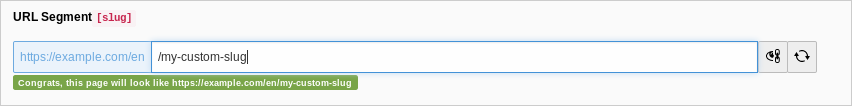
\includegraphics[width=0.80\linewidth]{BackendUserInterface/89115b-AutoSlugUpdateAndRedirectCreationOnSlugChange.png}
	\end{figure}

	\begin{itemize}
		\item Od TYPO3 v10.1, dve akcije sprečavaju da se ovo dogodi:

			\begin{itemize}
				\item slug-ovi za podstranice su automatski ažurirani
				\item redirekcije sa starih na nove URL-ove su kreirane
			\end{itemize}

	\end{itemize}

\end{frame}

% ------------------------------------------------------------------------------
% Feature | 89115 | Auto slug update and redirect creation on slug change

\begin{frame}[fragile]
	\frametitle{Administratorski interfejs}
	\framesubtitle{Slug unapredjenja i redirekcije (2)}

	\begin{itemize}
		\item Korisnici administratorskog interfejsa su informisani o ovim akcijama
			i oni mogu da vrate izmene na staro sa jednim klikom na dugme ako je potrebno:

	\end{itemize}

	\begin{figure}
		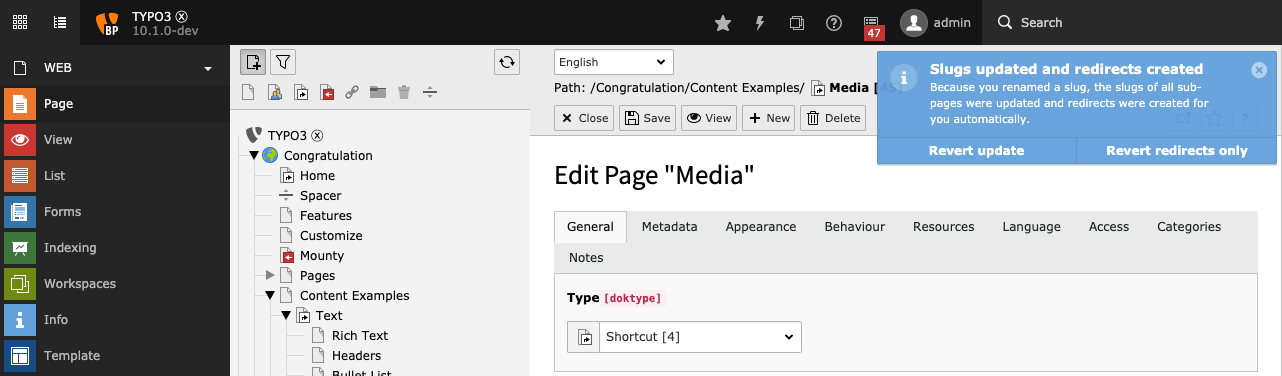
\includegraphics[width=0.80\linewidth]{BackendUserInterface/89115c-AutoSlugUpdateAndRedirectCreationOnSlugChange.png}
	\end{figure}

\end{frame}

% ------------------------------------------------------------------------------
% Feature | 85918 | Hide in menu / Show in menu entry for pages in context menu

\begin{frame}[fragile]
	\frametitle{Administratorski interfejs}
	\framesubtitle{Sakrij/Prikaži u meniuju}

	Nova stavka je dodata u kontekstualni meni da prikaže/sakrije stranice u meniju.

	\begin{figure}
		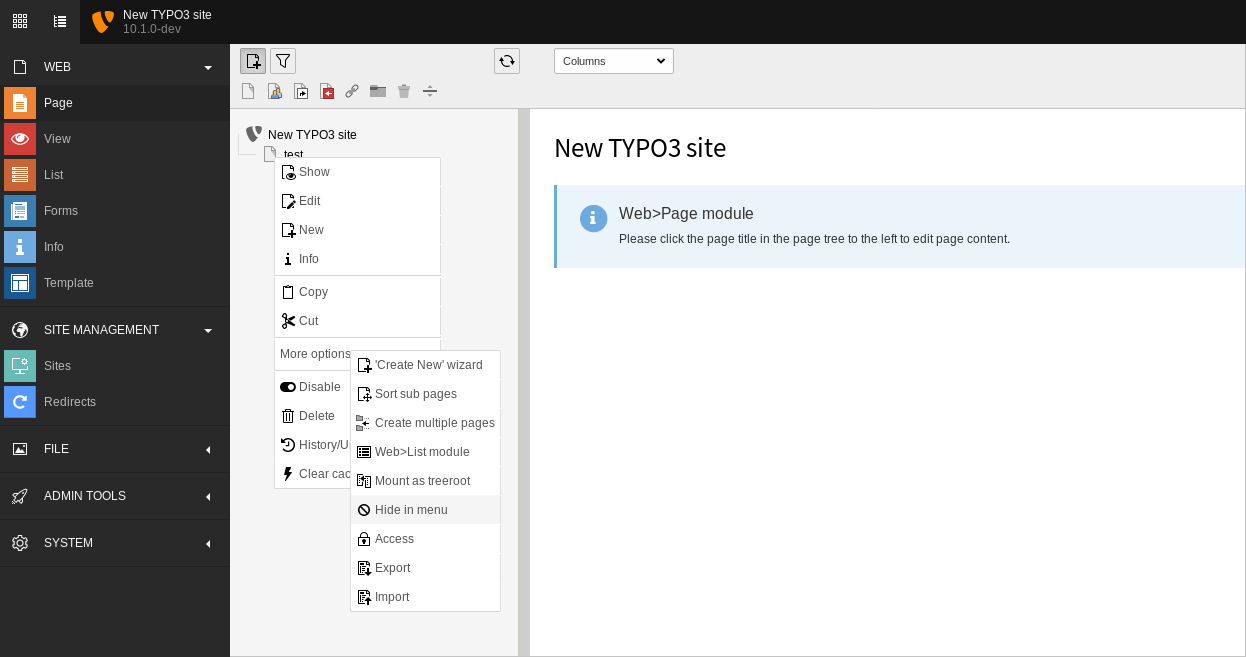
\includegraphics[width=0.80\linewidth]{BackendUserInterface/85918-HideShowInMenu-InContextMenu.png}
	\end{figure}

\end{frame}

% ------------------------------------------------------------------------------
